%%%%%%%%%%%%%%%%%%%%%%%%%%%%%%%%%%%%%%%%%
% Beamer Presentation
% LaTeX Template
% Version 1.0 (10/11/12)
%
% This template has been downloaded from:
% http://www.LaTeXTemplates.com
%
% License:
% CC BY-NC-SA 3.0 (http://creativecommons.org/licenses/by-nc-sa/3.0/)
%
%%%%%%%%%%%%%%%%%%%%%%%%%%%%%%%%%%%%%%%%%

%----------------------------------------------------------------------------------------
%	PACKAGES AND THEMES
%----------------------------------------------------------------------------------------

\documentclass{beamer}

\mode<presentation> {

% The Beamer class comes with a number of default slide themes
% which change the colors and layouts of slides. Below this is a list
% of all the themes, uncomment each in turn to see what they look like.

%\usetheme{default}
%\usetheme{AnnArbor}
%\usetheme{Antibes}
%\usetheme{Bergen}
%\usetheme{Berkeley}
%\usetheme{Berlin}
%\usetheme{Boadilla}
%\usetheme{CambridgeUS}
%\usetheme{Copenhagen}
%\usetheme{Darmstadt}
%\usetheme{Dresden}
%\usetheme{Frankfurt}
%\usetheme{Goettingen}
%\usetheme{Hannover}punto
%\usetheme{Ilmenau}
%\usetheme{JuanLesPins}punto
%\usetheme{Luebeck}
%\usetheme{Madrid}punto
%\usetheme{Malmoe}
%\usetheme{Marburg}
%\usetheme{Montpellier}punto
%\usetheme{PaloAlto}punto
%\usetheme{Pittsburgh}punto
%\usetheme{Rochester}punto
\usetheme{Singapore}
%\usetheme{Szeged}
%\usetheme{Warsaw}

% As well as themes, the Beamer class has a number of color themes
% for any slide theme. Uncomment each of these in turn to see how it
% changes the colors of your current slide theme.

%\usecolortheme{albatross}fondo azul
%\usecolortheme{beaver}titulos rojos
%\usecolortheme{beetle}fondo gris
%\usecolortheme{crane} resaltado amarillo
%\usecolortheme{dolphin} titulos azules
%\usecolortheme{dove} titulos negros
%\usecolortheme{fly} fondo gris, titulos blancos
%\usecolortheme{lily} ??
%\usecolortheme{orchid} ??
\usecolortheme{rose} %punto
%\usecolortheme{seagull} adornos gris
%\usecolortheme{seahorse} partes gris
%\usecolortheme{whale} partes azul
%\usecolortheme{wolverine} resalto amarillo

%\setbeamertemplate{footline} % To remove the footer line in all slides uncomment this line
\setbeamertemplate{footline}[page number] % To replace the footer line in all slides with a simple slide count uncomment this line

\setbeamertemplate{navigation symbols}{} % To remove the navigation symbols from the bottom of all slides uncomment this line
}

\usepackage{graphicx} % Allows including images
\usepackage{booktabs} % Allows the use of \toprule, \midrule and \bottomrule in tables
\usepackage{listings}
\usepackage{xcolor}
\usepackage{color}
%\usepackage[utf8]{inputenc}
%\usepackage[spanish]{babel}

\colorlet{punct}{red!60!black}
\definecolor{background}{HTML}{EEEEEE}
\definecolor{delim}{RGB}{25,134,57}
%\definecolor{delim}{RGB}{20,105,176}
\colorlet{numb}{magenta!60!black}

\lstdefinelanguage{json}{
    basicstyle=\normalfont\ttfamily,
    numbers=left,
    numberstyle=\scriptsize,
    stepnumber=1,
    numbersep=8pt,
    showstringspaces=false,
    breaklines=true,
    frame=lines,
    backgroundcolor=\color{background},
    literate=
     *{0}{{{\color{numb}0}}}{1}
      {1}{{{\color{numb}1}}}{1}
      {2}{{{\color{numb}2}}}{1}
      {3}{{{\color{numb}3}}}{1}
      {4}{{{\color{numb}4}}}{1}
      {5}{{{\color{numb}5}}}{1}
      {6}{{{\color{numb}6}}}{1}
      {7}{{{\color{numb}7}}}{1}
      {8}{{{\color{numb}8}}}{1}
      {9}{{{\color{numb}9}}}{1}
      {:}{{{\color{punct}{:}}}}{1}
      {,}{{{\color{punct}{,}}}}{1}
      {\{}{{{\color{delim}{\{}}}}{1}
      {\}}{{{\color{delim}{\}}}}}{1}
      {[}{{{\color{delim}{[}}}}{1}
      {]}{{{\color{delim}{]}}}}{1},
}
%----------------------------------------------------------------------------------------
%	TITLE PAGE
%----------------------------------------------------------------------------------------

\title[CodingDojo]{Coding Dojo} % The short title appears at the bottom of every slide, the full title is only on the title page

\author{Jesse Javier Cogollo Alvarez} % Your name
\institute[EAFIT] % Your institution as it will appear on the bottom of every slide, may be shorthand to save space
{
Developer by passion \\ % Your institution for the title page
\medskip
\textit{email: cogollo87@gmail.com} \\~\\
\textit{Agile Open Space Popay\'an}
}
%\date{\today} % Date, can be changed to a custom date
\begin{document}

\begin{frame}
\titlepage % Print the title page as the first slide
\end{frame}

\begin{frame}
\frametitle{Contenido} % Table of contents slide, comment this block out to remove it
\tableofcontents % Throughout your presentation, if you choose to use \section{} and \subsection{} commands, these will automatically be printed on this slide as an overview of your presentation
\end{frame}

%----------------------------------------------------------------------------------------
%	PRESENTATION SLIDES
%----------------------------------------------------------------------------------------

%------------------------------------------------
\section{TDD - Test Driven Development} % Sections can be created in order to organize your presentation into discrete blocks, all sections and subsections are automatically printed in the table of contents as an overview of the talk
%------------------------------------------------
\begin{frame}
\frametitle{Que es TDD}
Es una practica de programaci\'on orientada a objetos. Que se basa en la repetici\'on 
de un \textbf{ciclo} de desarrollo muy corto.
{\color{blue}\url{http://en.wikipedia.org/wiki/Test-driven_development/}}
\\~\\
Kent Beck

{\color{blue}\url{http://en.wikipedia.org/wiki/Kent_Beck}}

\begin{figure}
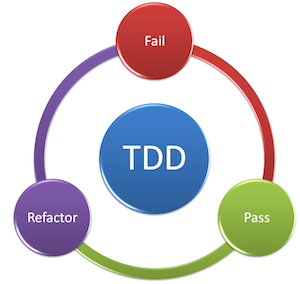
\includegraphics[width=0.3\linewidth]{tdd.png}
\end{figure}
\end{frame}

%------------------------------------------------
\begin{frame}
\frametitle{Ciclo TDD}
\begin{columns}[c] % The "c" option specifies centered vertical alignment while the "t" option is used for top vertical alignment

\column{.45\textwidth} % Left column and width
\begin{enumerate}
\item \textbf{Escribir prueba}
\item[•]	
\item[•]	
\item[•]	
\item[•]	
\item[•]	
\end{enumerate}

\column{.5\textwidth} % Right column and width
\begin{figure}
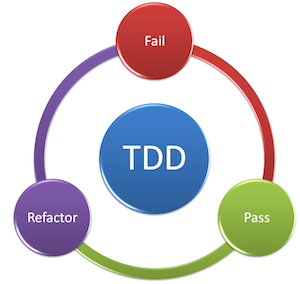
\includegraphics[width=0.9\linewidth]{tdd.png}
\end{figure}
\end{columns}
\end{frame}

%------------------------------------------------

\begin{frame}
\frametitle{Ciclo TDD}
\begin{columns}[c] % The "c" option specifies centered vertical alignment while the "t" option is used for top vertical alignment

\column{.45\textwidth} % Left column and width
\begin{enumerate}
\item \textbf{Escribir prueba}
\item {\color{red}\textbf{Correr Pruebas}}
\item[•]	
\item[•]	
\item[•]	
\item[•]	
\end{enumerate}

\column{.5\textwidth} % Right column and width
\begin{figure}
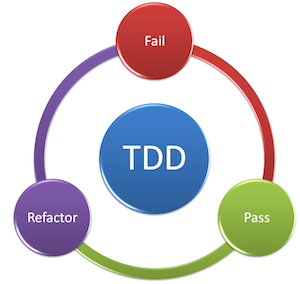
\includegraphics[width=0.9\linewidth]{tdd.png}
\end{figure}
\end{columns}
\end{frame}

%------------------------------------------------
\begin{frame}
\frametitle{Ciclo TDD}
\begin{columns}[c] % The "c" option specifies centered vertical alignment while the "t" option is used for top vertical alignment

\column{.45\textwidth} % Left column and width
\begin{enumerate}
\item \textbf{Escribir prueba}
\item {\color{red}\textbf{Correr Pruebas}}
\item \textbf{Escribir Codigo}
\item[•]	
\item[•]	
\item[•]	
\end{enumerate}

\column{.5\textwidth} % Right column and width
\begin{figure}
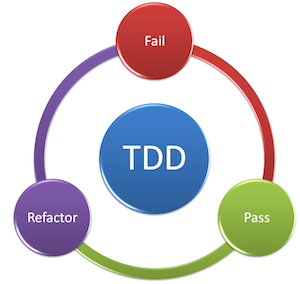
\includegraphics[width=0.9\linewidth]{tdd.png}
\end{figure}
\end{columns}
\end{frame}

%------------------------------------------------
\begin{frame}
\frametitle{Ciclo TDD}
\begin{columns}[c] % The "c" option specifies centered vertical alignment while the "t" option is used for top vertical alignment

\column{.45\textwidth} % Left column and width
\begin{enumerate}
\item \textbf{Escribir prueba}
\item {\color{red}\textbf{Correr Pruebas}}
\item \textbf{Escribir Codigo}
\item {\color{green}\textbf{Correr Pruebas}}
\item[•]	
\item[•]	
\end{enumerate}

\column{.5\textwidth} % Right column and width
\begin{figure}
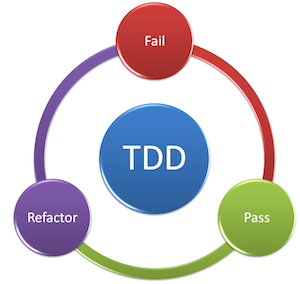
\includegraphics[width=0.9\linewidth]{tdd.png}
\end{figure}
\end{columns}
\end{frame}

%------------------------------------------------
\begin{frame}
\frametitle{Ciclo TDD}
\begin{columns}[c] % The "c" option specifies centered vertical alignment while the "t" option is used for top vertical alignment

\column{.45\textwidth} % Left column and width
\begin{enumerate}
\item \textbf{Escribir prueba}
\item {\color{red}\textbf{Correr Pruebas}}
\item \textbf{Escribir Codigo}
\item {\color{green}\textbf{Correr Pruebas}}
\item \textbf{Refactoriar Codigo}
\item[•]	
\end{enumerate}

\column{.5\textwidth} % Right column and width
\begin{figure}
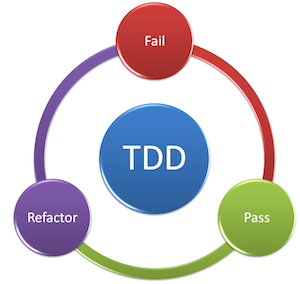
\includegraphics[width=0.9\linewidth]{tdd.png}
\end{figure}
\end{columns}
\end{frame}

%------------------------------------------------
\begin{frame}
\frametitle{Ciclo TDD}
\begin{columns}[c] % The "c" option specifies centered vertical alignment while the "t" option is used for top vertical alignment

\column{.45\textwidth} % Left column and width
\begin{enumerate}
\item \textbf{Escribir prueba}
\item {\color{red}\textbf{Correr Pruebas}}
\item \textbf{Escribir Codigo}
\item {\color{green}\textbf{Correr Pruebas}}
\item \textbf{Refactoriar Codigo}
\item {\color{purple}\textbf{Correr Pruebas}}
\end{enumerate}

\column{.5\textwidth} % Right column and width
\begin{figure}
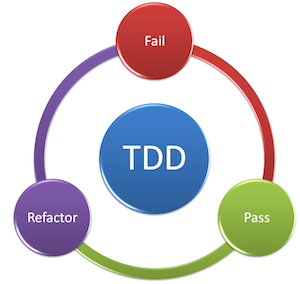
\includegraphics[width=0.9\linewidth]{tdd.png}
\end{figure}
\end{columns}
\end{frame}

%------------------------------------------------
\begin{frame}
\frametitle{Mejores practicas}
\begin{columns}[c] % The "c" option specifies centered vertical alignment while the "t" option is used for top vertical alignment

\column{.45\textwidth} % Left column and width
\begin{enumerate}
\item \textbf{Estructura - AAA(siglas en ingles)}
\item[•]	
\item[•]	
\item[•]	
\end{enumerate}

\column{.5\textwidth} % Right column and width
Preparar - Arrange
\end{columns}
\end{frame}

%------------------------------------------------
\begin{frame}
\frametitle{Mejores practicas}
\begin{columns}[c] % The "c" option specifies centered vertical alignment while the "t" option is used for top vertical alignment

\column{.45\textwidth} % Left column and width
\begin{enumerate}
\item \textbf{Estructura - AAA(siglas en ingles)}
\item[•]	
\item[•]	
\item[•]	
\end{enumerate}

\column{.5\textwidth} % Right column and width
Preparar - Arrange

Actuar - Act
\end{columns}
\end{frame}

%------------------------------------------------
\begin{frame}
\frametitle{Mejores practicas}
\begin{columns}[c] % The "c" option specifies centered vertical alignment while the "t" option is used for top vertical alignment

\column{.45\textwidth} % Left column and width
\begin{enumerate}
\item \textbf{Estructura - AAA(siglas en ingles)}
\item[•]	
\item[•]	
\item[•]	
\end{enumerate}

\column{.5\textwidth} % Right column and width
Preparar - Arrange

Actuar - Act

Afirmar - Assert
\end{columns}
\end{frame}

%------------------------------------------------
\begin{frame}
\frametitle{Mejores practicas}
\begin{columns}[c] % The "c" option specifies centered vertical alignment while the "t" option is used for top vertical alignment

\column{.45\textwidth} % Left column and width
\begin{enumerate}
\item \textbf{Estructura - AAA(siglas en ingles)}
\item \textbf{Desacoplaje y simplicidad}
\item[•]	
\item[•]	

\end{enumerate}

\column{.5\textwidth} % Right column and width
No agregar logica de negocio en las pruebas.

cada prueba realiza una unica prueba.
\end{columns}
\end{frame}

%------------------------------------------------
\begin{frame}
\frametitle{Mejores practicas}
\begin{columns}[c] % The "c" option specifies centered vertical alignment while the "t" option is used for top vertical alignment

\column{.45\textwidth} % Left column and width
\begin{enumerate}
\item \textbf{Estructura - AAA(siglas en ingles)}
\item \textbf{Desacoplaje y simplicidad}
\item \textbf{Compartir}
\item[•]	

\end{enumerate}

\column{.5\textwidth} % Right column and width
Realiza conding dojos con tus companeros y/o amigos.

Previene adquirir malos habitos y ayuda a mejorar nuestras tecnicas de desarrollo.
\end{columns}
\end{frame}

%------------------------------------------------
\begin{frame}
\frametitle{Mejores practicas}
\begin{columns}[c] % The "c" option specifies centered vertical alignment while the "t" option is used for top vertical alignment

\column{.45\textwidth} % Left column and width
\begin{enumerate}
\item \textbf{Estructura - AAA(siglas en ingles)}
\item \textbf{Desacoplaje y simplicidad}
\item \textbf{Compartir}
\item \textbf{Dar importancia}

\end{enumerate}

\column{.5\textwidth} % Right column and width
Tomar conciencia de las pruebas como parte del desarrollo de software, evitando deuda tecnica en el desarrollo de software.
\end{columns}
\end{frame}

\section{Coding Dojo}
%------------------------------------------------
\begin{frame}
\frametitle{Coding Dojo (para informaticos)}
\begin{columns}[c] % The "c" option specifies centered vertical alignment while the "t" option is used for top vertical alignment

\column{.45\textwidth} % Left column and width
\begin{enumerate}
\item \textbf{Que es}
\item[•]
\item[•]
\item[•]
\item[•]

\end{enumerate}

\column{.5\textwidth} % Right column and width
Es un lugar para aprender y divertirse mientras programamos.
\end{columns}
\end{frame}
%------------------------------------------------

\begin{frame}
\frametitle{Coding Dojo}
\begin{columns}[c] % The "c" option specifies centered vertical alignment while the "t" option is used for top vertical alignment

\column{.45\textwidth} % Left column and width
\begin{enumerate}
\item \textbf{Que es}
\item \textbf{estilo 1}
\item[•]
\item[•]
\item[•]

\end{enumerate}

\column{.5\textwidth} % Right column and width
\textbf{randori} Muchos programadores un problema.
\end{columns}
\end{frame}
%------------------------------------------------

\begin{frame}
\frametitle{Coding Dojo}
\begin{columns}[c] % The "c" option specifies centered vertical alignment while the "t" option is used for top vertical alignment

\column{.45\textwidth} % Left column and width
\begin{enumerate}
\item \textbf{Que es}
\item \textbf{estilo 1}
\item \textbf{estilo 2}
\item[•]
\item[•]

\end{enumerate}

\column{.5\textwidth} % Right column and width
Pair programming en paralelo. (Cyberdojo.org)
\end{columns}
\end{frame}
%------------------------------------------------

\begin{frame}
\frametitle{Coding Dojo}
\begin{columns}[c] % The "c" option specifies centered vertical alignment while the "t" option is used for top vertical alignment

\column{.45\textwidth} % Left column and width
\begin{enumerate}
\item \textbf{Que es}
\item \textbf{estilo 1}
\item \textbf{estilo 2}
\item \textbf{estilo 3}
\item[•]

\end{enumerate}

\column{.5\textwidth} % Right column and width
Trabajando bajo presi\'on. (Extreme startup)
\end{columns}
\end{frame}
%------------------------------------------------

\begin{frame}
\frametitle{Coding Dojo}
\begin{columns}[c] % The "c" option specifies centered vertical alignment while the "t" option is used for top vertical alignment

\column{.45\textwidth} % Left column and width
\begin{enumerate}
\item \textbf{Que es}
\item \textbf{estilo 1}
\item \textbf{estilo 2}
\item \textbf{estilo 3}
\item \textbf{recursos}
\end{enumerate}

\column{.5\textwidth} % Right column and width
\begin{itemize}
\item Un computador con el ambiente de desarrollo listo. 
\item un projector 
\item un lugar para runirse
\item un facilitador
\item entre 4 y muchos programadores con ganas de divertirse.
\end{itemize}
\end{columns}
\end{frame}
%------------------------------------------------
\begin{frame}
\frametitle{Redes sociales}
\begin{columns}[c] % The "c" option specifies centered vertical alignment while the "t" option is used for top vertical alignment

\column{.45\textwidth} % Left column and width
\begin{enumerate}
\item \textbf{Meetup}
\item[•]	
\item[•]	
\item[•]	
\item[•]	
\end{enumerate}

\column{.5\textwidth} % Right column and width
%\begin{figure}
%
\includegraphics[width=0.5\linewidth]{meetup.png}
%\end{figure}
{\color{blue}/MongoDB-Medellin}
\\~\\
{\color{blue}\url{http://goo.gl/fw5Gyh}}
\end{columns}
\end{frame}
%------------------------------------------------

\begin{frame}
\frametitle{Redes sociales}
\begin{columns}[c] % The "c" option specifies centered vertical alignment while the "t" option is used for top vertical alignment

\column{.45\textwidth} % Left column and width
\begin{enumerate}
\item Meetup
\item \textbf{Twitter}
\item[•]	
\item[•]	
\item[•]	
\end{enumerate}

\column{.5\textwidth} % Right column and width
%\begin{figure}
%
\includegraphics[width=0.5\linewidth]{twitter.png}
%\end{figure}
{\color{blue}@jessecogollo}
\\~\\
{\color{blue}\url{http://goo.gl/gdCAjF}}
\end{columns}
\end{frame}
%------------------------------------------------

\begin{frame}
\frametitle{Redes sociales}
\begin{columns}[c] % The "c" option specifies centered vertical alignment while the "t" option is used for top vertical alignment

\column{.45\textwidth} % Left column and width
\begin{enumerate}
\item Meetup
\item Twitter
\item \textbf{Facebook}
\item[•]	
\item[•]	
\end{enumerate}

\column{.5\textwidth} % Right column and width
%\begin{figure}
%
\includegraphics[width=0.5\linewidth]{facebook.png}
%\end{figure}
{\color{blue}/jessecogollo}
\\~\\
{\color{blue}\url{http://goo.gl/Q1JnXQ}}
\end{columns}
\end{frame}
%------------------------------------------------	
\begin{frame}
\frametitle{Redes sociales}
\begin{columns}[c] % The "c" option specifies centered vertical alignment while the "t" option is used for top vertical alignment

\column{.45\textwidth} % Left column and width
\begin{enumerate}
\item Meetup
\item Twitter
\item Facebook
\item Google Plus
\item \textbf{Lista de correo}
\item[•]	
\end{enumerate}

\column{.5\textwidth} % Right column and width
%\begin{figure}
%
\includegraphics[width=0.5\linewidth]{gmail.png}
%\end{figure}
{\color{blue}+ correo}
\\~\\
{\color{blue}\url{http://goo.gl/FJvrjT}}
\end{columns}
\end{frame}
%------------------------------------------------	
\begin{frame}
\frametitle{Redes sociales}
\begin{columns}[c] % The "c" option specifies centered vertical alignment while the "t" option is used for top vertical alignment

\column{.45\textwidth} % Left column and width
\begin{enumerate}
\item Meetup
\item Twitter
\item Facebook
\item Google Plus
\item Lista de correo
\item \textbf{Grupo de estudio}
\end{enumerate}

\column{.5\textwidth} % Right column and width
%\begin{figure}
%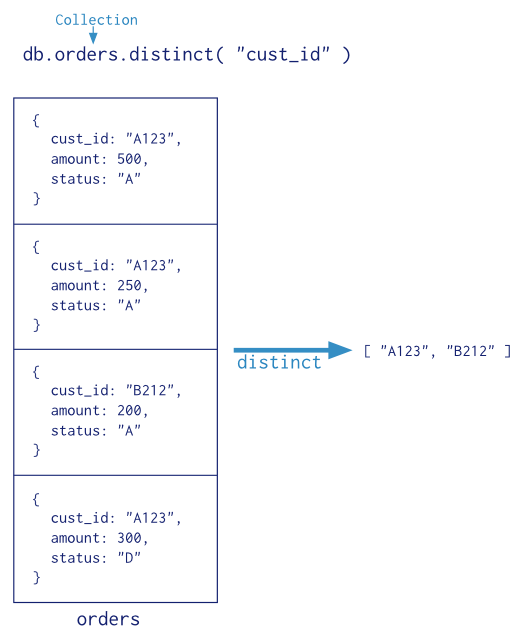
\includegraphics[width=0.5\linewidth]{distinct.png}
%\end{figure}
{\color{blue}Formulario grupo de estudio}
\\~\\
{\color{blue}\url{http://goo.gl/7ALdst}}
\end{columns}
\end{frame}
%------------------------------------------------	
\begin{frame}
\frametitle{Donde aprender}
\begin{columns}[c] % The "c" option specifies centered vertical alignment while the "t" option is used for top vertical alignment
\column{.45\textwidth} % Left column and width
\begin{enumerate}
\item \textbf{Organizar un coding dojo}
\item[•]
\item[•]
\item[•]
\item[•]
\end{enumerate}

\column{.5\textwidth} % Right column and width
%\begin{figure}
%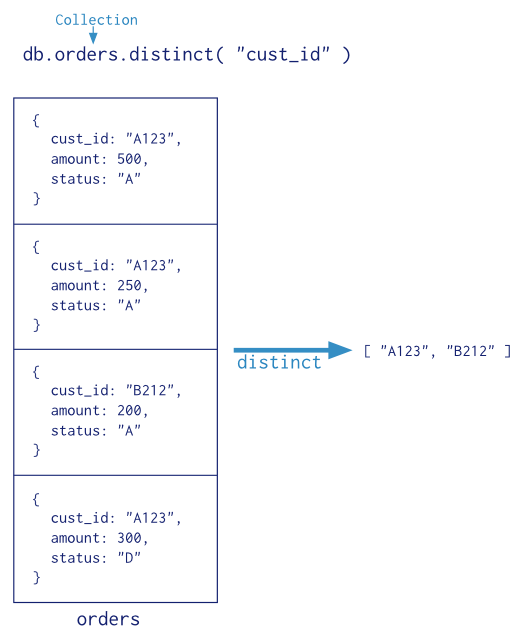
\includegraphics[width=0.5\linewidth]{distinct.png}
%\end{figure}
{\color{blue}\url{http://johannesbrodwall.com/2011/12/18/how-to-start-a-coding-dojo/}}
\end{columns}
\end{frame}
%------------------------------------------------	
\begin{frame}
\frametitle{Donde aprender}
\begin{columns}[c] % The "c" option specifies centered vertical alignment while the "t" option is used for top vertical alignment
\column{.45\textwidth} % Left column and width
\begin{enumerate}
\item Organizar un coding dojo
\item \textbf{Cyber dojo}
\item[•]
\item[•]
\item[•]
\end{enumerate}

\column{.5\textwidth} % Right column and width
%\begin{figure}
%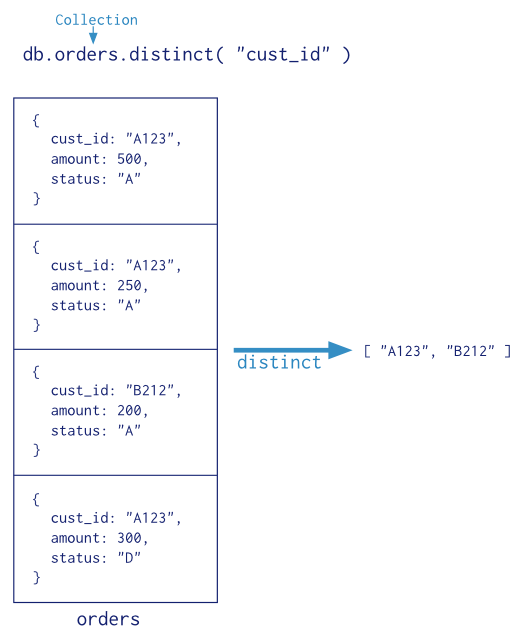
\includegraphics[width=0.5\linewidth]{distinct.png}
%\end{figure}
{\color{blue}\url{http://cyber-dojo.org/}}
\end{columns}
\end{frame}
%------------------------------------------------	
\begin{frame}
\frametitle{Donde aprender}
\begin{columns}[c] % The "c" option specifies centered vertical alignment while the "t" option is used for top vertical alignment
\column{.45\textwidth} % Left column and width
\begin{enumerate}
\item Organizar un coding dojo
\item Cyber dojo
\item \textbf{Codingdojo}
\item[•]
\item[•]
\end{enumerate}

\column{.5\textwidth} % Right column and width
%\begin{figure}
%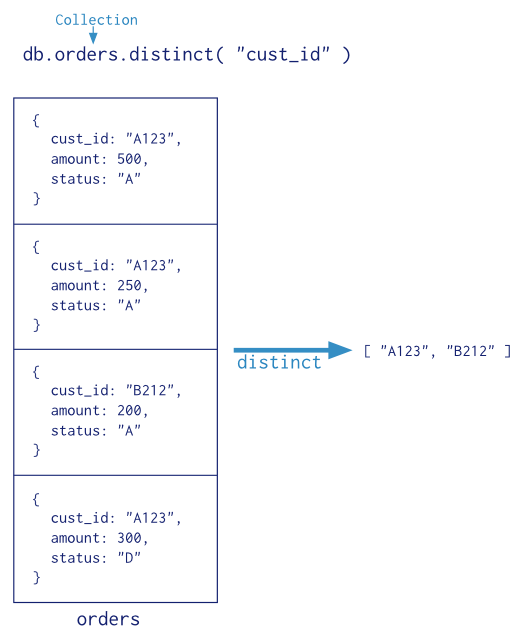
\includegraphics[width=0.5\linewidth]{distinct.png}
%\end{figure}
{\color{blue}\url{http://www.codingdojo.org/}}
\end{columns}
\end{frame}
%------------------------------------------------	
\begin{frame}
\frametitle{Donde aprender}
\begin{columns}[c] % The "c" option specifies centered vertical alignment while the "t" option is used for top vertical alignment
\column{.45\textwidth} % Left column and width
\begin{enumerate}
\item Organizar un coding dojo
\item Cyber dojo
\item Codingdojo
\item \textbf{Ejercicios}
\item[•]
\end{enumerate}

\column{.5\textwidth} % Right column and width
%\begin{figure}
%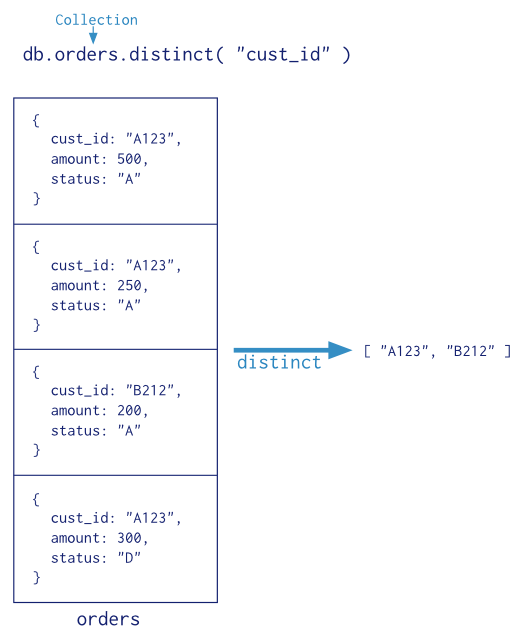
\includegraphics[width=0.5\linewidth]{distinct.png}
%\end{figure}
{\color{blue}\url{http://rosettacode.org/wiki/Category:Programming_Tasks}}
\end{columns}
\end{frame}
%------------------------------------------------	
\begin{frame}
\frametitle{Donde aprender}
\begin{columns}[c] % The "c" option specifies centered vertical alignment while the "t" option is used for top vertical alignment
\column{.45\textwidth} % Left column and width
\begin{enumerate}
\item Organizar un coding dojo
\item Cyber dojo
\item Codingdojo
\item Ejercicios
\item \textbf{Mas ejercicios}
\end{enumerate}

\column{.5\textwidth} % Right column and width
%\begin{figure}
%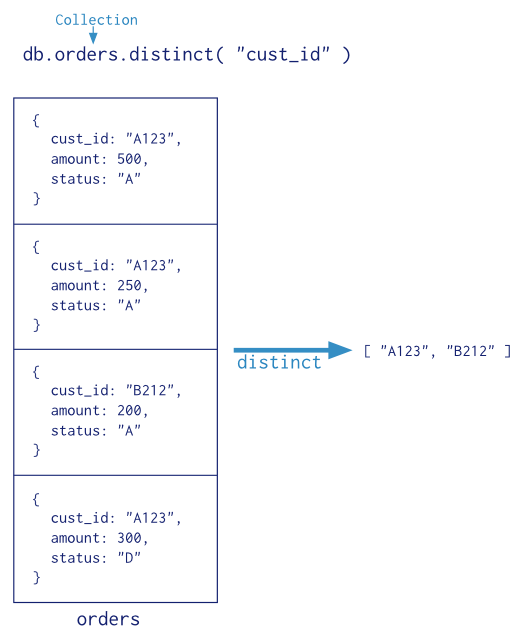
\includegraphics[width=0.5\linewidth]{distinct.png}
%\end{figure}
{\color{blue}\url{http://brendan.enrick.com/post/Coding-Katas-and-Exercises}}
\end{columns}
\end{frame}
%------------------------------------------------
\begin{frame}
\frametitle{Preguntas}
%\begin{figure}
%
\includegraphics[width=0.4\linewidth]{preguntas.png}
%\end{figure}
\end{frame}
%------------------------------------------------
\begin{frame}
\frametitle{Empecemos...}
\begin{figure}

\includegraphics[width=0.4\linewidth]{happy.png}
\end{figure}
\end{frame}
%------------------------------------------------
\begin{frame}
\Huge{\centerline{Gracias !!! =)}}
\end{frame}

%----------------------------------------------------------------------------------------

\end{document} 
